\begin{figure}[htbp]
  \centering

  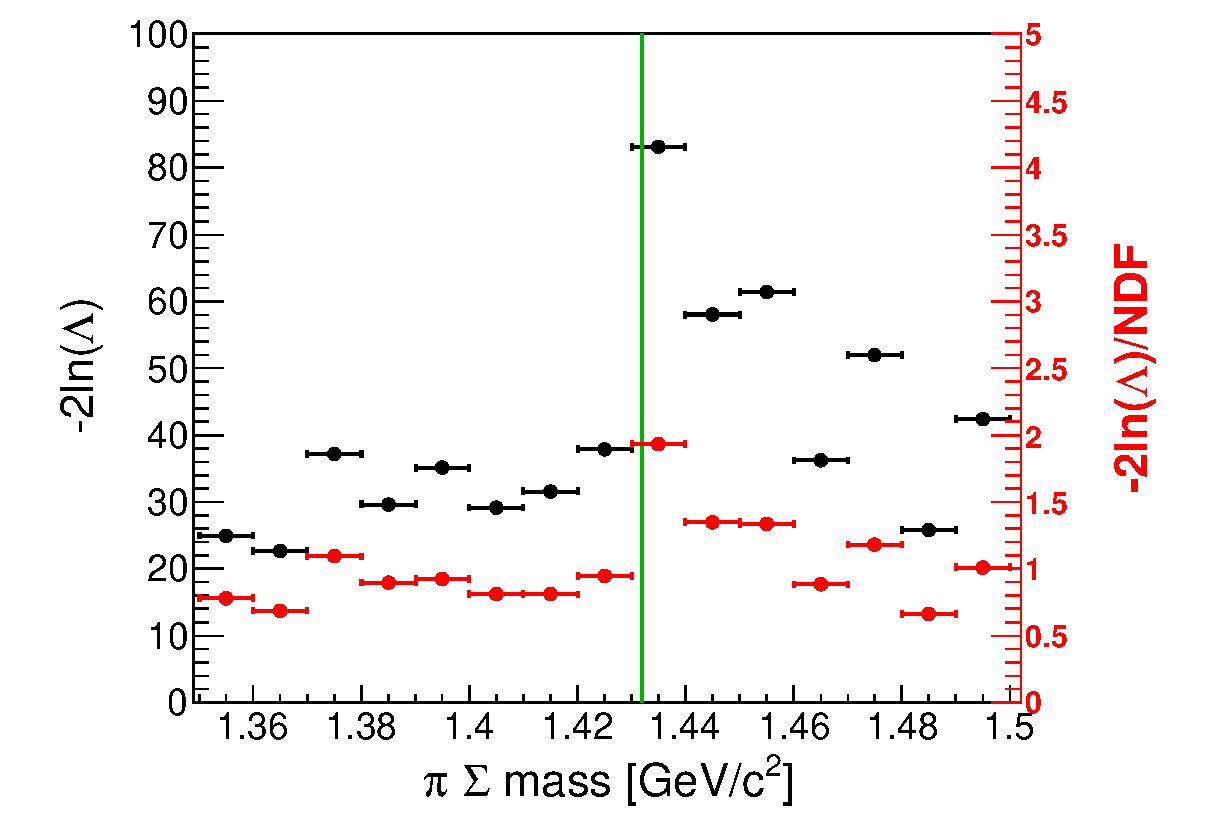
\includegraphics[width=8cm]{../pic/Dron/tempFit_KNpi_MM_Chi2.eps}
  \caption{
    This figure shows the template fitting results of −2$\ln(\Lambda)$ and −2$\ln(\Lambda)/NDF$
    for the separation of $\pi^-\Sigma^+$ and $\pi^+\Sigma^-$ modes in each $d(K^-, n)$ bin.
    Black and red lines indicate −2$\ln(\Lambda)$ and −2$\ln(\Lambda)/NDF$, respectively.
    The horizontal axis represents the $(K^-, n)$ bin.
  }
  \label{fig:tempFit_KNpi_Chi2}
\end{figure}
